\section{Theorie}
\label{sec:Theorie}
\subsection{Die allgemeine Relaxationsgleichung}
Unter einer Relaxationserscheinung versteht man allgemein das Phänomen, wenn
 ein System aus seinem Ausgangszustand entfernt wird und es sich nicht oszillatorisch
 in diesen zurückbewegt.Die Änderungsrate der betrachteten Größe A verläuft dabei
 in der Regel proportional zur bis zum Ausgangszustand verbleibenden Entfernung. Daher
  verläuft die Näherung auch nur asymptotisch. Für diese
 Bewegung gilt dann:
 \begin{equation}
   \frac{dA}{dt} = c[A(t)-A(\infty)]
 \end{equation}
Womit man zur allgemeinen Bewegungsgleichung des Systems gelangt:
\begin{equation}
  A(t) = A(\infty)+[A(0)-A(\infty)]e^{ct}
\end{equation}
Damit A einen endlichen Endpunkt hat muss $ c < 0$ gelten.

\subsection{Relaxationsverhalten bei einem RC-Glied}

Für das RC-Glied in Abb. 1 gilt nach den Kirchhoffschen Regeln:
\begin{equation}
  \frac{dQ}{dt} = -\frac{1}{RC}Q(t)
\end{equation}
Die Gleichung zeigt sich dasselbe Muster wie der allgemeine Fall.
\begin{figure}[H]
  \centering
  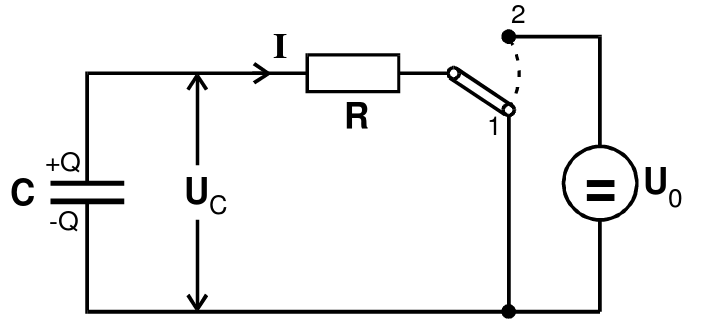
\includegraphics[width=\linewidth-200pt,height=\textheight-200pt,keepaspectratio]{content/RC_Kreis1.png}
  \caption{RC-Kreis}
  \label{fig:RC_Kreis1}
\end{figure}

Mit der Randbedingung $ Q(\infty)=0$ folgt dann für den Entladevorgang:
\begin{equation}
  Q(t) = Q(0) \cdot e^{-\frac{t}{RC}}
\end{equation}
Mit den Randbedingungen $Q(0) = 0 $ und $Q(\infty) = CU_0$ folgt analog für
den Aufladevorgang:
\begin{equation}
  Q(t) = CU_0 \left(1-e^{-\frac{t}{RC}}\right)
\end{equation}
RC wird als Zeitkonstante des Relaxationsvorgangs bezeichnet und in der Regel mit
 $\tau$ abgekürzt. So ändert sich die Ladung auf dem Kondensator in einem Zeitraum
 $\Delta$ T = $\tau$ ca. um den Faktor 0,368.

 \subsection{Relaxationsphänomene aufgrund einer periodischen Auslenkung aus der Gleichgewichtslage}

 Solange für die Frequenz der Wechselspannung $ f_{Antrieb} \ll \frac{1}{2RC\pi} $ gilt, lässt sich
 $U_C(t)$ für jeden Zeitpunkt t mit U(t) gleichsetzen.Bei höheren Antriebsfrequenzen
 kann sich der Kondensator jedoch nichtmehr vollständig über den Widerstand
  auf- bzw. entladen und bleibt hinter dem Verlauf der Generatorspannung zurück.
  Es stellt sich also eine Phasenverschiebung zwischen $U_c$ und $U_{Antrieb}$ ein.

\begin{figure}[H]
  \centering

  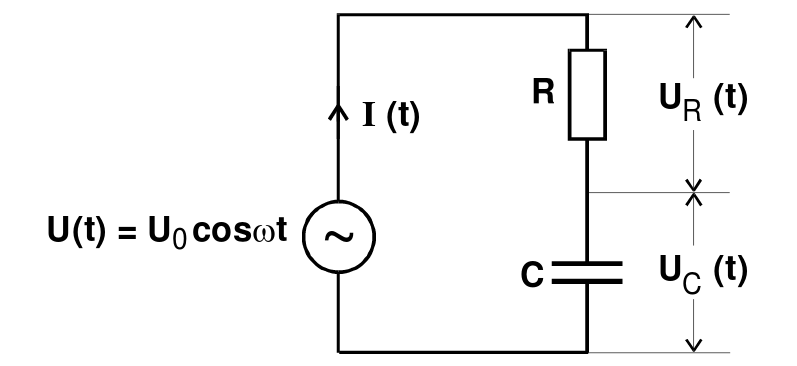
\includegraphics[width=\linewidth-200pt,height=\textheight-200pt,keepaspectratio]{content/RC_Kreis2.png}
  \caption{periodisch angetriebener RC-Kreis}
  \label{fig:RC_Kreis2}
\end{figure}

  Mit dem Ansatz
  \begin{equation}
  U_C(t) = A(\omega)cos(\omega t+\varphi(\omega))
  \end{equation}
  folgt dann für $A(\omega)$ und $\varphi(\omega)$:
  \begin{equation}
    A(\omega) = \frac{U_0}{\sqrt{1+\omega^2R^2C^2}}
  \end{equation}
  \begin{equation}
    \varphi(\omega) = arctan(-RC \cdot \omega)
  \end{equation}

Es lässt sich erkennen das die Amplitude für $\omega \to 0$ gegen $U_0$ läuft, für
$\omega \to \infty$ verschwindet. Aufgrund dieser Eigenschaft findet das RC-Glied als
 Tiefpass Verwendung, da Wechselspannungen mit Frequenzen $f_{Antrieb} \gg \frac{1}{RC}$
  unghindert passieren können, hochfrequente jedoch immer weiter abgeschwächt werden.
  Der einzige Nachteil für Anwendungen besteht darin das die Schwächung nur eine $\omega^{-1}$
  Abhängigkeit besizt und damit oft zu flach verläuft.

\subsection{Der RC-Kreis als Integrator}

Ein RC-Kreis bietet auch die Möglichkeit, eine zeitlich veränderliche Spannung U(t), die
wie in Abb. 2 angeschlossen ist, zu integrieren. Es folgt aus den kirchhoffschen Gesetzen:
\begin{equation}
  U(t) = RC\frac{dU_C}{dt}+U_C(t)
\end{equation}
Wählt man nun eine Frequenz mit $f_{Antrieb} \gg \frac{1}{RC}$ und hat
$|U_C| \ll |U_R|$ und $|U_C| \ll |U_{Antrieb}|$ kann der zusätzliche Term "$+ U_C(t)$"
 vernachlässigt werden. Hiermit folgt dann:
\begin{equation}
U_C(t) = \frac{1}{RC}\int_{0}^{t} U(t') \symup{d}t'
\end{equation}
